\chapter{Cusomization}

Three ways to customize Emacs:
\begin{enumerate}
\item Options
\item Custom
\item Lisp code
\end{enumerate}

No matter what method you use, though, the .emacs startup file is modified.
Custom modifies it for you when you save settings through that interface.
The Options menu invokes Custom behind the scenes; when you choose Save Options, Custom again modifies .emacs.

\section{Hide Tool Bar}
Refer to the Figure: \ref{fig:hide-tool-bar}.

\begin{figure}[!ht]
  \label{fig:hide-tool-bar}
  \centering
  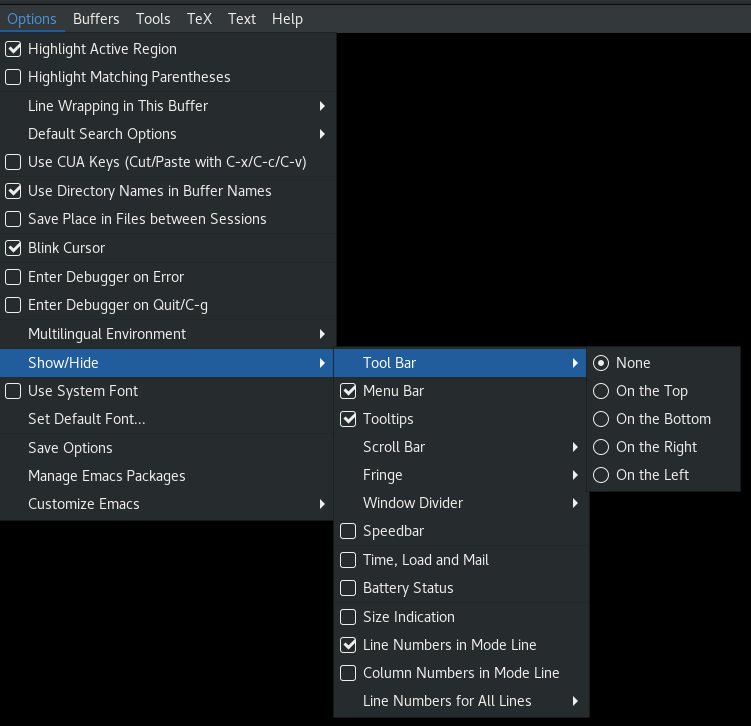
\includegraphics[width=0.6\textwidth]{hide-tool-bar.png}
  \caption{Hide tool bar}
\end{figure}

After the hiding, remember to press the \verb|Save Options|.
\clearpage


\section{Theme}
Refer to the Figure: \ref{fig:theme}.

\begin{figure}[!ht]
  \label{fig:theme}
  \centering
  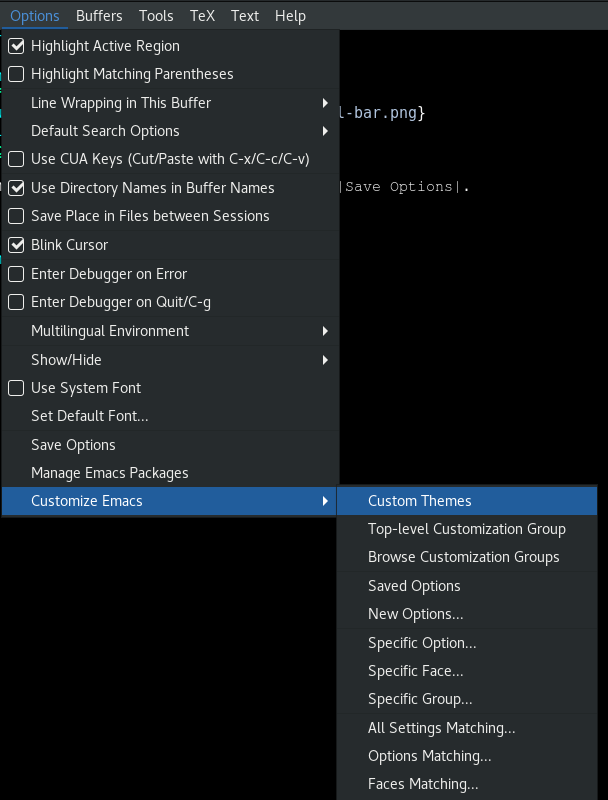
\includegraphics[width=0.8\textwidth]{theme.png}
  \caption{Theme}
\end{figure}
After the hiding, remember to press the \verb|Save Options|.
\clearpage

\section{Package Repository}
\href{https://www.melpa.org/}{MELPA} (Milkypostman's Emacs Lisp Package Archive) is a emacs lisp package repository.

Add the following Emacs Lisp code into you \verb|init.el| or \verb|.emacs| file.
% \lstset{language=Lisp}
\begin{lstlisting}
  (require 'package)
  % (add-to-list 'package-archives '("melpa" . "https://melpa.org/packages/") t)
  % ;; Comment/uncomment this line to enable MELPA Stable if desired.  See `package-archive-priorities`
  % ;; and `package-pinned-packages`. Most users will not need or want to do this.
  % ;;(add-to-list 'package-archives '("melpa-stable" . "https://stable.melpa.org/packages/") t)
  % (package-initialize)
\end{lstlisting}


\section{Some Customization}
\lstset{language=Lisp}
\begin{lstlisting}
;; install packages
(defvar my-packages
  '(better-defaults			; set up some better Emacs defaults
    material-theme			; Theme
    )
  )

;; scans the list in my-packages
;; if the package listed is not already installed, install it
(mapc #'(lambda (package)
	  (unless (package-installed-p package)
	    (package-install package)))
      my-packages)


;; basic cusomization
(setq inhibit-startup-message t)	; hide the startup message
(load-theme 'material t)		; load material theme
(global-linum-mode t)			; enable line numbers globally
\end{lstlisting}


\section{Customize Default Directory}
\lstset{language=Lisp}
\begin{lstlisting}
  (setq default-directory "~/")
\end{lstlisting}


\section{Enter Full Screen on Startup}

\begin{lstlisting}
  (toggle-frame-fullscreen)		; enter fullscreen on startup
\end{lstlisting}


\section{Set Default Font}

The formal configuration is:
\begin{enumerate}
\item Options $\rightarrow$ Set Default Font
\item After you select you font, press Options $\rightarrow$ Save Options
\end{enumerate}


However this configuration does not work on my MacOS.
Here's the oprations that work on MacOS:
\begin{enumerate}
\item Options $\rightarrow$ Set Default Font
\item M-x desribe-font
\item Copy the name (Here is my first line ``name (opened by): -*-Menlo-normal-normal-normal-*-9-*-*-*-m-0-iso10646-1'')
\item add the the Elisp code ``(add-to-list 'default-frame-alist '(font . "-*-Menlo-normal-normal-normal-*-9-*-*-*-m-0-iso10646-1"))''
\end{enumerate}

\section{Treemacs}


Treemacs is a file and project explorer similar to NeoTree or vim’s NerdTree, but largely inspired by the Project Explorer in Eclipse.
It shows the file system outlines of your projects in a simple tree layout allowing quick navigation and exploration, while also possessing basic file management utilities.

\lstset{language=Elisp}
\begin{lstlisting}
  M-x package-install RET
  treemacs* RET
\end{lstlisting}

After the installation, type \verb|M-x treemacs| to evoke the treemacs.

The effect is as shown in Figure \ref{fig:treemacs}
\begin{figure}[!ht]
  \centering
  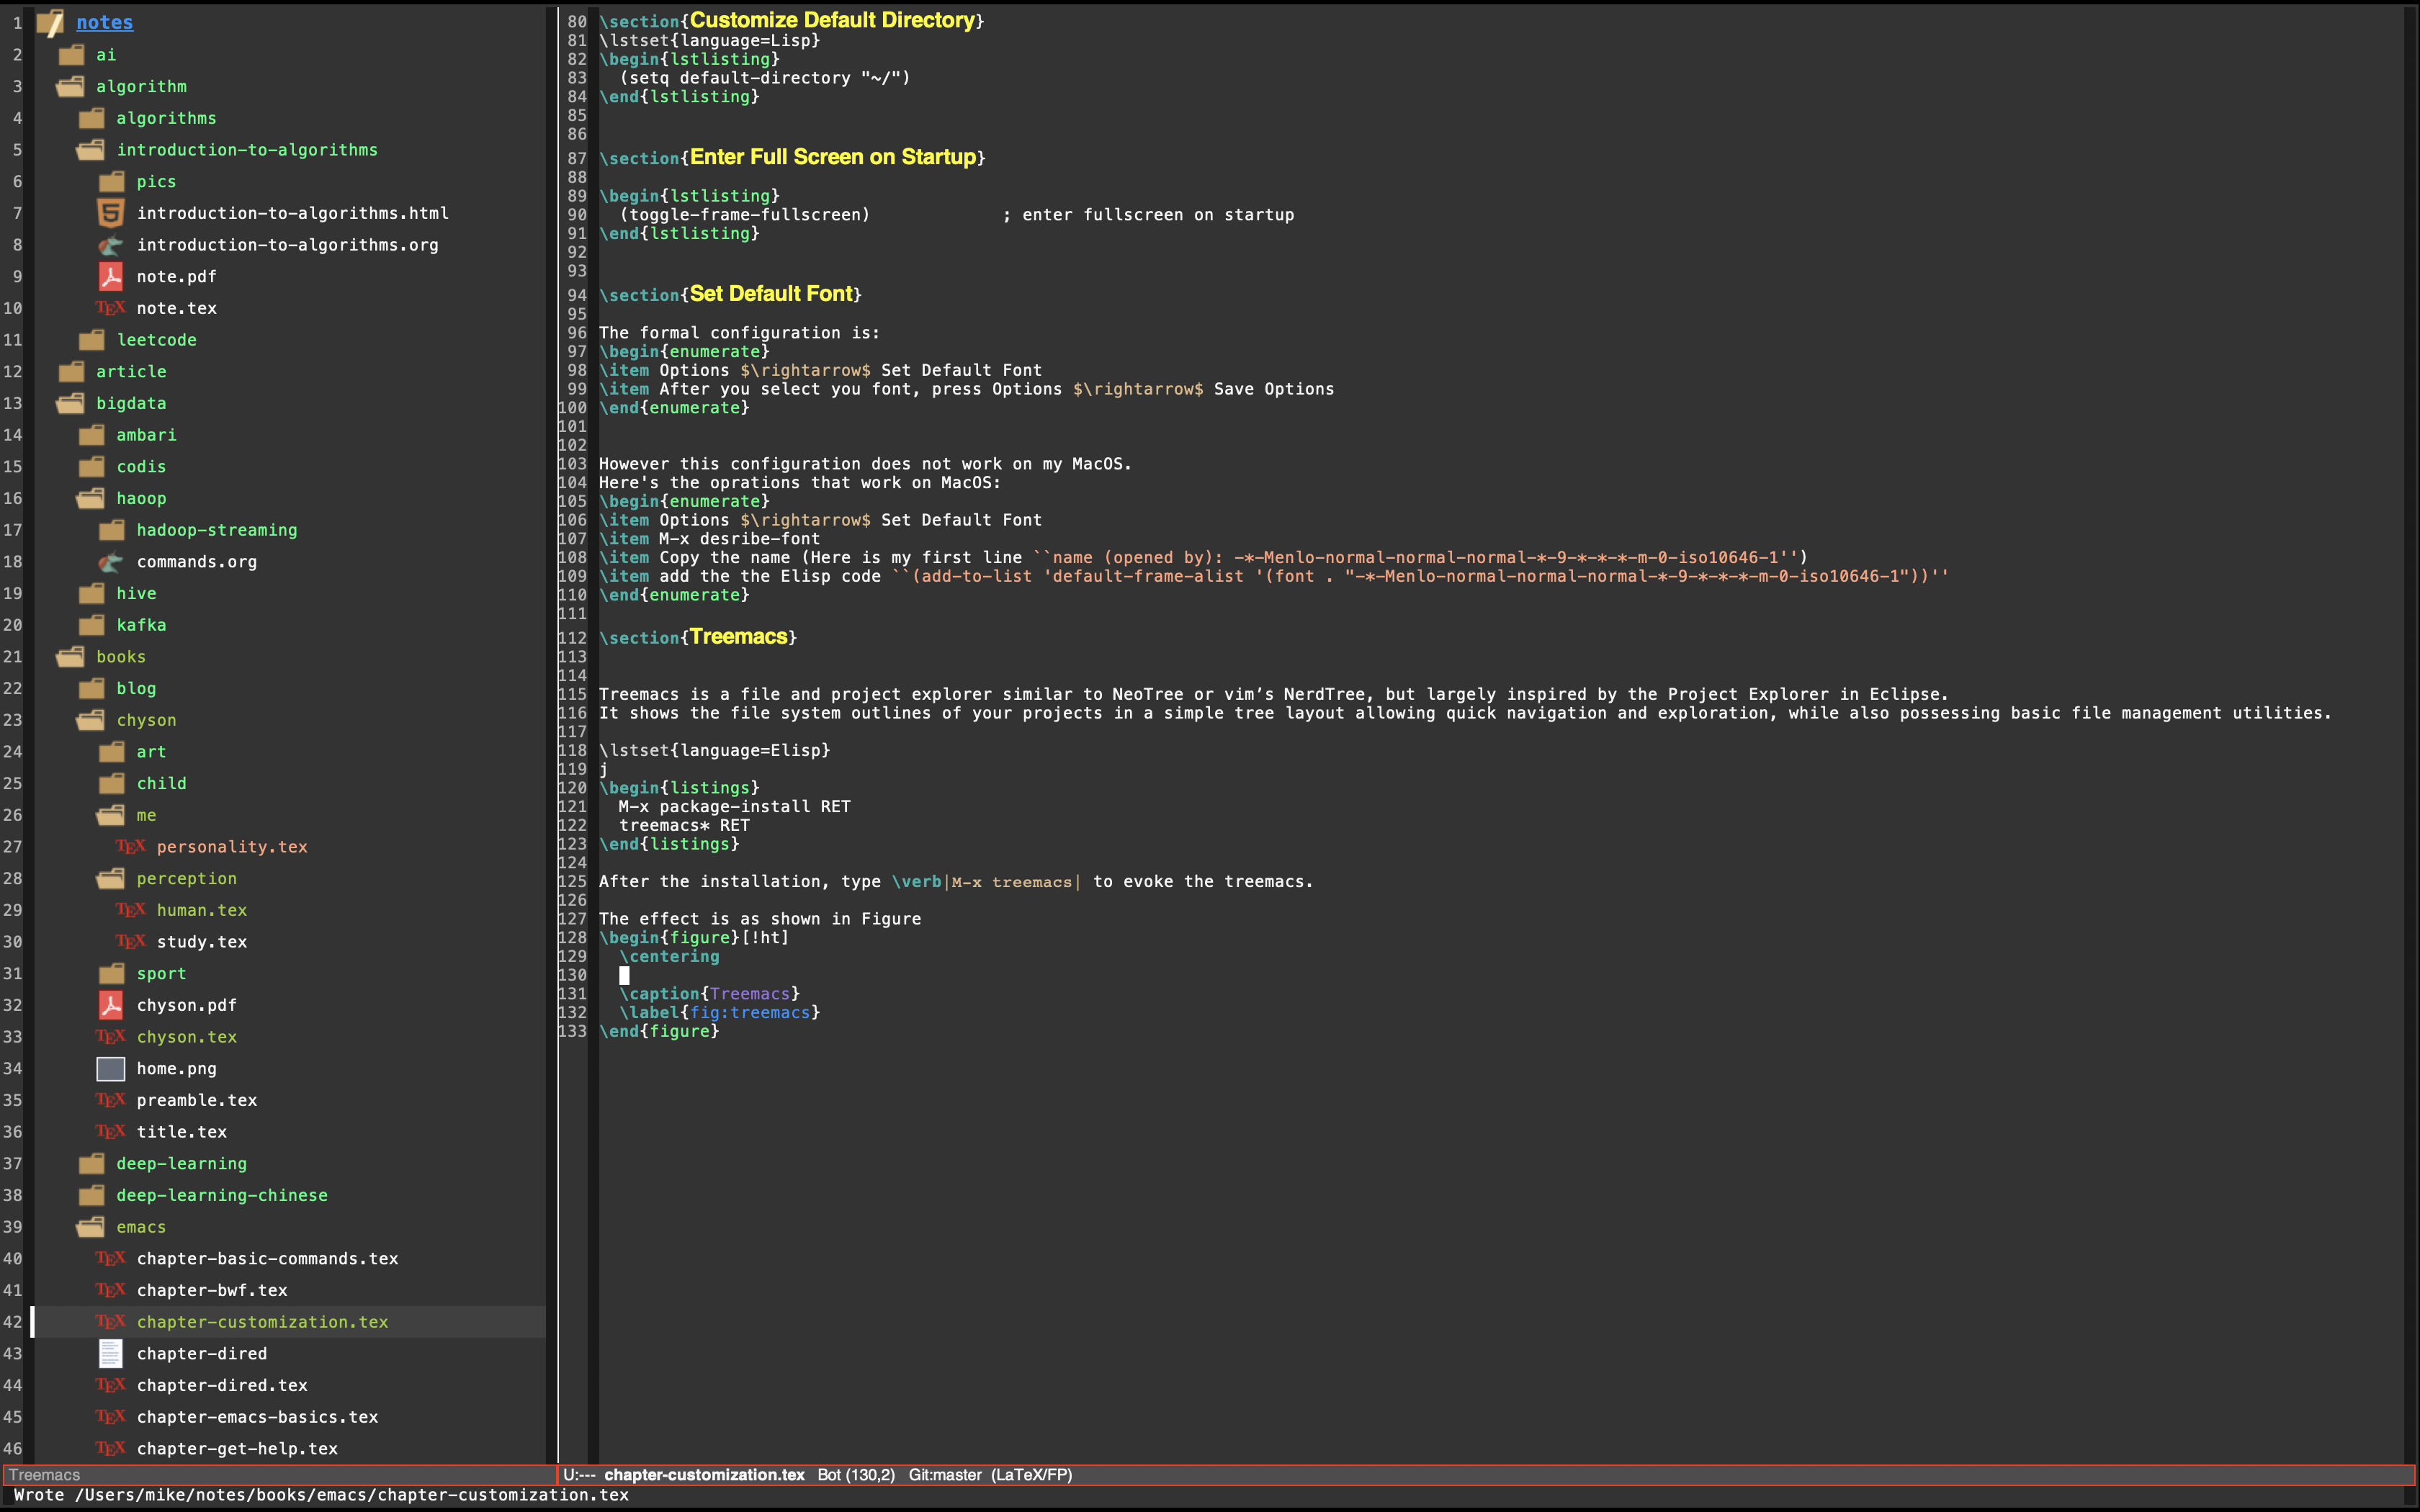
\includegraphics[width=\textwidth]{treemacs}
  \caption{Treemacs}
  \label{fig:treemacs}
\end{figure}
